
%% bare_jrnl.tex
%% V1.4
%% 2012/12/27
%% by Michael Shell
%% see http://www.michaelshell.org/
%% for current contact information.
%%
%% This is a skeleton file demonstrating the use of IEEEtran.cls
%% (requires IEEEtran.cls version 1.8 or later) with an IEEE journal paper.
%%
%% Support sites:
%% http://www.michaelshell.org/tex/ieeetran/
%% http://www.ctan.org/tex-archive/macros/latex/contrib/IEEEtran/
%% and
%% http://www.ieee.org/



% *** Authors should verify (and, if needed, correct) their LaTeX system  ***
% *** with the testflow diagnostic prior to trusting their LaTeX platform ***
% *** with production work. IEEE's font choices can trigger bugs that do  ***
% *** not appear when using other class files.                            ***
% The testflow support page is at:
% http://www.michaelshell.org/tex/testflow/


%%*************************************************************************
%% Legal Notice:
%% This code is offered as-is without any warranty either expressed or
%% implied; without even the implied warranty of MERCHANTABILITY or
%% FITNESS FOR A PARTICULAR PURPOSE! 
%% User assumes all risk.
%% In no event shall IEEE or any contributor to this code be liable for
%% any damages or losses, including, but not limited to, incidental,
%% consequential, or any other damages, resulting from the use or misuse
%% of any information contained here.
%%
%% All comments are the opinions of their respective authors and are not
%% necessarily endorsed by the IEEE.
%%
%% This work is distributed under the LaTeX Project Public License (LPPL)
%% ( http://www.latex-project.org/ ) version 1.3, and may be freely used,
%% distributed and modified. A copy of the LPPL, version 1.3, is included
%% in the base LaTeX documentation of all distributions of LaTeX released
%% 2003/12/01 or later.
%% Retain all contribution notices and credits.
%% ** Modified files should be clearly indicated as such, including  **
%% ** renaming them and changing author support contact information. **
%%
%% File list of work: IEEEtran.cls, IEEEtran_HOWTO.pdf, bare_adv.tex,
%%                    bare_conf.tex, bare_jrnl.tex, bare_jrnl_compsoc.tex,
%%                    bare_jrnl_transmag.tex
%%*************************************************************************

% Note that the a4paper option is mainly intended so that authors in
% countries using A4 can easily print to A4 and see how their papers will
% look in print - the typesetting of the document will not typically be
% affected with changes in paper size (but the bottom and side margins will).
% Use the testflow package mentioned above to verify correct handling of
% both paper sizes by the user's LaTeX system.
%
% Also note that the "draftcls" or "draftclsnofoot", not "draft", option
% should be used if it is desired that the figures are to be displayed in
% draft mode.
%
\documentclass[journal]{IEEEtran}
%
% If IEEEtran.cls has not been installed into the LaTeX system files,
% manually specify the path to it like:
% \documentclass[journal]{../sty/IEEEtran}





% Some very useful LaTeX packages include:
% (uncomment the ones you want to load)


% *** MISC UTILITY PACKAGES ***
%
%\usepackage{ifpdf}
% Heiko Oberdiek's ifpdf.sty is very useful if you need conditional
% compilation based on whether the output is pdf or dvi.
% usage:
% \ifpdf
%   % pdf code
% \else
%   % dvi code
% \fi
% The latest version of ifpdf.sty can be obtained from:
% http://www.ctan.org/tex-archive/macros/latex/contrib/oberdiek/
% Also, note that IEEEtran.cls V1.7 and later provides a builtin
% \ifCLASSINFOpdf conditional that works the same way.
% When switching from latex to pdflatex and vice-versa, the compiler may
% have to be run twice to clear warning/error messages.






% *** CITATION PACKAGES ***
%
%\usepackage{cite}
% cite.sty was written by Donald Arseneau
% V1.6 and later of IEEEtran pre-defines the format of the cite.sty package
% \cite{} output to follow that of IEEE. Loading the cite package will
% result in citation numbers being automatically sorted and properly
% "compressed/ranged". e.g., [1], [9], [2], [7], [5], [6] without using
% cite.sty will become [1], [2], [5]--[7], [9] using cite.sty. cite.sty's
% \cite will automatically add leading space, if needed. Use cite.sty's
% noadjust option (cite.sty V3.8 and later) if you want to turn this off
% such as if a citation ever needs to be enclosed in parenthesis.
% cite.sty is already installed on most LaTeX systems. Be sure and use
% version 4.0 (2003-05-27) and later if using hyperref.sty. cite.sty does
% not currently provide for hyperlinked citations.
% The latest version can be obtained at:
% http://www.ctan.org/tex-archive/macros/latex/contrib/cite/
% The documentation is contained in the cite.sty file itself.






% *** GRAPHICS RELATED PACKAGES ***
%
\ifCLASSINFOpdf
  % \usepackage[pdftex]{graphicx}
  % declare the path(s) where your graphic files are
  % \graphicspath{{../pdf/}{../jpeg/}}
  % and their extensions so you won't have to specify these with
  % every instance of \includegraphics
  % \DeclareGraphicsExtensions{.pdf,.jpeg,.png}
\else
  % or other class option (dvipsone, dvipdf, if not using dvips). graphicx
  % will default to the driver specified in the system graphics.cfg if no
  % driver is specified.
  % \usepackage[dvips]{graphicx}
  % declare the path(s) where your graphic files are
  % \graphicspath{{../eps/}}
  % and their extensions so you won't have to specify these with
  % every instance of \includegraphics
  % \DeclareGraphicsExtensions{.eps}
\fi
% graphicx was written by David Carlisle and Sebastian Rahtz. It is
% required if you want graphics, photos, etc. graphicx.sty is already
% installed on most LaTeX systems. The latest version and documentation
% can be obtained at: 
% http://www.ctan.org/tex-archive/macros/latex/required/graphics/
% Another good source of documentation is "Using Imported Graphics in
% LaTeX2e" by Keith Reckdahl which can be found at:
% http://www.ctan.org/tex-archive/info/epslatex/
%
% latex, and pdflatex in dvi mode, support graphics in encapsulated
% postscript (.eps) format. pdflatex in pdf mode supports graphics
% in .pdf, .jpeg, .png and .mps (metapost) formats. Users should ensure
% that all non-photo figures use a vector format (.eps, .pdf, .mps) and
% not a bitmapped formats (.jpeg, .png). IEEE frowns on bitmapped formats
% which can result in "jaggedy"/blurry rendering of lines and letters as
% well as large increases in file sizes.
%
% You can find documentation about the pdfTeX application at:
% http://www.tug.org/applications/pdftex





% *** MATH PACKAGES ***
%
%\usepackage[cmex10]{amsmath}
% A popular package from the American Mathematical Society that provides
% many useful and powerful commands for dealing with mathematics. If using
% it, be sure to load this package with the cmex10 option to ensure that
% only type 1 fonts will utilized at all point sizes. Without this option,
% it is possible that some math symbols, particularly those within
% footnotes, will be rendered in bitmap form which will result in a
% document that can not be IEEE Xplore compliant!
%
% Also, note that the amsmath package sets \interdisplaylinepenalty to 10000
% thus preventing page breaks from occurring within multiline equations. Use:
%\interdisplaylinepenalty=2500
% after loading amsmath to restore such page breaks as IEEEtran.cls normally
% does. amsmath.sty is already installed on most LaTeX systems. The latest
% version and documentation can be obtained at:
% http://www.ctan.org/tex-archive/macros/latex/required/amslatex/math/





% *** SPECIALIZED LIST PACKAGES ***
%
%\usepackage{algorithmic}
% algorithmic.sty was written by Peter Williams and Rogerio Brito.
% This package provides an algorithmic environment fo describing algorithms.
% You can use the algorithmic environment in-text or within a figure
% environment to provide for a floating algorithm. Do NOT use the algorithm
% floating environment provided by algorithm.sty (by the same authors) or
% algorithm2e.sty (by Christophe Fiorio) as IEEE does not use dedicated
% algorithm float types and packages that provide these will not provide
% correct IEEE style captions. The latest version and documentation of
% algorithmic.sty can be obtained at:
% http://www.ctan.org/tex-archive/macros/latex/contrib/algorithms/
% There is also a support site at:
% http://algorithms.berlios.de/index.html
% Also of interest may be the (relatively newer and more customizable)
% algorithmicx.sty package by Szasz Janos:
% http://www.ctan.org/tex-archive/macros/latex/contrib/algorithmicx/




% *** ALIGNMENT PACKAGES ***
%
%\usepackage{array}
% Frank Mittelbach's and David Carlisle's array.sty patches and improves
% the standard LaTeX2e array and tabular environments to provide better
% appearance and additional user controls. As the default LaTeX2e table
% generation code is lacking to the point of almost being broken with
% respect to the quality of the end results, all users are strongly
% advised to use an enhanced (at the very least that provided by array.sty)
% set of table tools. array.sty is already installed on most systems. The
% latest version and documentation can be obtained at:
% http://www.ctan.org/tex-archive/macros/latex/required/tools/


% IEEEtran contains the IEEEeqnarray family of commands that can be used to
% generate multiline equations as well as matrices, tables, etc., of high
% quality.




% *** SUBFIGURE PACKAGES ***
%\ifCLASSOPTIONcompsoc
%  \usepackage[caption=false,font=normalsize,labelfont=sf,textfont=sf]{subfig}
%\else
%  \usepackage[caption=false,font=footnotesize]{subfig}
%\fi
% subfig.sty, written by Steven Douglas Cochran, is the modern replacement
% for subfigure.sty, the latter of which is no longer maintained and is
% incompatible with some LaTeX packages including fixltx2e. However,
% subfig.sty requires and automatically loads Axel Sommerfeldt's caption.sty
% which will override IEEEtran.cls' handling of captions and this will result
% in non-IEEE style figure/table captions. To prevent this problem, be sure
% and invoke subfig.sty's "caption=false" package option (available since
% subfig.sty version 1.3, 2005/06/28) as this is will preserve IEEEtran.cls
% handling of captions.
% Note that the Computer Society format requires a larger sans serif font
% than the serif footnote size font used in traditional IEEE formatting
% and thus the need to invoke different subfig.sty package options depending
% on whether compsoc mode has been enabled.
%
% The latest version and documentation of subfig.sty can be obtained at:
% http://www.ctan.org/tex-archive/macros/latex/contrib/subfig/




% *** FLOAT PACKAGES ***
%
%\usepackage{fixltx2e}
% fixltx2e, the successor to the earlier fix2col.sty, was written by
% Frank Mittelbach and David Carlisle. This package corrects a few problems
% in the LaTeX2e kernel, the most notable of which is that in current
% LaTeX2e releases, the ordering of single and double column floats is not
% guaranteed to be preserved. Thus, an unpatched LaTeX2e can allow a
% single column figure to be placed prior to an earlier double column
% figure. The latest version and documentation can be found at:
% http://www.ctan.org/tex-archive/macros/latex/base/


%\usepackage{stfloats}
% stfloats.sty was written by Sigitas Tolusis. This package gives LaTeX2e
% the ability to do double column floats at the bottom of the page as well
% as the top. (e.g., "\begin{figure*}[!b]" is not normally possible in
% LaTeX2e). It also provides a command:
%\fnbelowfloat
% to enable the placement of footnotes below bottom floats (the standard
% LaTeX2e kernel puts them above bottom floats). This is an invasive package
% which rewrites many portions of the LaTeX2e float routines. It may not work
% with other packages that modify the LaTeX2e float routines. The latest
% version and documentation can be obtained at:
% http://www.ctan.org/tex-archive/macros/latex/contrib/sttools/
% Do not use the stfloats baselinefloat ability as IEEE does not allow
% \baselineskip to stretch. Authors submitting work to the IEEE should note
% that IEEE rarely uses double column equations and that authors should try
% to avoid such use. Do not be tempted to use the cuted.sty or midfloat.sty
% packages (also by Sigitas Tolusis) as IEEE does not format its papers in
% such ways.
% Do not attempt to use stfloats with fixltx2e as they are incompatible.
% Instead, use Morten Hogholm'a dblfloatfix which combines the features
% of both fixltx2e and stfloats:
%
% \usepackage{dblfloatfix}
% The latest version can be found at:
% http://www.ctan.org/tex-archive/macros/latex/contrib/dblfloatfix/




%\ifCLASSOPTIONcaptionsoff
%  \usepackage[nomarkers]{endfloat}
% \let\MYoriglatexcaption\caption
% \renewcommand{\caption}[2][\relax]{\MYoriglatexcaption[#2]{#2}}
%\fi
% endfloat.sty was written by James Darrell McCauley, Jeff Goldberg and 
% Axel Sommerfeldt. This package may be useful when used in conjunction with 
% IEEEtran.cls'  captionsoff option. Some IEEE journals/societies require that
% submissions have lists of figures/tables at the end of the paper and that
% figures/tables without any captions are placed on a page by themselves at
% the end of the document. If needed, the draftcls IEEEtran class option or
% \CLASSINPUTbaselinestretch interface can be used to increase the line
% spacing as well. Be sure and use the nomarkers option of endfloat to
% prevent endfloat from "marking" where the figures would have been placed
% in the text. The two hack lines of code above are a slight modification of
% that suggested by in the endfloat docs (section 8.4.1) to ensure that
% the full captions always appear in the list of figures/tables - even if
% the user used the short optional argument of \caption[]{}.
% IEEE papers do not typically make use of \caption[]'s optional argument,
% so this should not be an issue. A similar trick can be used to disable
% captions of packages such as subfig.sty that lack options to turn off
% the subcaptions:
% For subfig.sty:
% \let\MYorigsubfloat\subfloat
% \renewcommand{\subfloat}[2][\relax]{\MYorigsubfloat[]{#2}}
% However, the above trick will not work if both optional arguments of
% the \subfloat command are used. Furthermore, there needs to be a
% description of each subfigure *somewhere* and endfloat does not add
% subfigure captions to its list of figures. Thus, the best approach is to
% avoid the use of subfigure captions (many IEEE journals avoid them anyway)
% and instead reference/explain all the subfigures within the main caption.
% The latest version of endfloat.sty and its documentation can obtained at:
% http://www.ctan.org/tex-archive/macros/latex/contrib/endfloat/
%
% The IEEEtran \ifCLASSOPTIONcaptionsoff conditional can also be used
% later in the document, say, to conditionally put the References on a 
% page by themselves.




% *** PDF, URL AND HYPERLINK PACKAGES ***
%
%\usepackage{url}
% url.sty was written by Donald Arseneau. It provides better support for
% handling and breaking URLs. url.sty is already installed on most LaTeX
% systems. The latest version and documentation can be obtained at:
% http://www.ctan.org/tex-archive/macros/latex/contrib/url/
% Basically, \url{my_url_here}.




% *** Do not adjust lengths that control margins, column widths, etc. ***
% *** Do not use packages that alter fonts (such as pslatex).         ***
% There should be no need to do such things with IEEEtran.cls V1.6 and later.
% (Unless specifically asked to do so by the journal or conference you plan
% to submit to, of course. )


% correct bad hyphenation here
\hyphenation{op-tical net-works semi-conduc-tor}
\usepackage{color}

\usepackage{graphicx}
\usepackage{braket}

\begin{document}
%
% paper title
% can use linebreaks \\ within to get better formatting as desired
% Do not put math or special symbols in the title.
\title{Making Quantum Leaps for Computation}
%
%
% author names and IEEE memberships
% note positions of commas and nonbreaking spaces ( ~ ) LaTeX will not break
% a structure at a ~ so this keeps an author's name from being broken across
% two lines.
% use \thanks{} to gain access to the first footnote area
% a separate \thanks must be used for each paragraph as LaTeX2e's \thanks
% was not built to handle multiple paragraphs
%

\author{Krysta~M.~Svore~and~Matthias~Troyer% <-this % stops a space
\thanks{K. Svore is with the Quantum Architectures and Computation Group, Microsoft Research, Redmond, WA (USA).}% <-this % stops a space
\thanks{M. Troyer is with the Institute for Theoretical Physics of ETH Zurich (Switzerland)  and with the Quantum Architectures and Computation Group, Microsoft Research, Redmond, WA (USA).}% <-this % stops a space
%\thanks{Manuscript received April 19, 2005; revised December 27, 2012.}
}

% note the % following the last \IEEEmembership and also \thanks - 
% these prevent an unwanted space from occurring between the last author name
% and the end of the author line. i.e., if you had this:
% 
% \author{....lastname \thanks{...} \thanks{...} }
%                     ^------------^------------^----Do not want these spaces!
%
% a space would be appended to the last name and could cause every name on that
% line to be shifted left slightly. This is one of those "LaTeX things". For
% instance, "\textbf{A} \textbf{B}" will typeset as "A B" not "AB". To get
% "AB" then you have to do: "\textbf{A}\textbf{B}"
% \thanks is no different in this regard, so shield the last } of each \thanks
% that ends a line with a % and do not let a space in before the next \thanks.
% Spaces after \IEEEmembership other than the last one are OK (and needed) as
% you are supposed to have spaces between the names. For what it is worth,
% this is a minor point as most people would not even notice if the said evil
% space somehow managed to creep in.



% The paper headers
\markboth{IEEE Computer}%
{Svore and Troyer: Quantum Computing}% The only time the second header will appear is for the odd numbered pages
% after the title page when using the twoside option.
% 
% *** Note that you probably will NOT want to include the author's ***
% *** name in the headers of peer review papers.                   ***
% You can use \ifCLASSOPTIONpeerreview for conditional compilation here if
% you desire.




% If you want to put a publisher's ID mark on the page you can do it like
% this:
%\IEEEpubid{0000--0000/00\$00.00~\copyright~2012 IEEE}
% Remember, if you use this you must call \IEEEpubidadjcol in the second
% column for its text to clear the IEEEpubid mark.



% use for special paper notices
%\IEEEspecialpapernotice{(Invited Paper)}




% make the title area
\maketitle

% As a general rule, do not put math, special symbols or citations
% in the abstract or keywords.
\begin{abstract}
The coming quantum revolution will overturn our notions of computational methods and devices. Still in early stages of development, quantum computers use the quantum mechanical properties of superposition and entanglement to solve problems that are likely to be forever out of reach of classical computers.  Already we have a diverse range of quantum algorithms that outperform their classical counterparts, from cryptography to chemistry and materials science. Quantum computers will operate as co-processors, receiving instructions from a stack of classical processors.  A scalable software stack is crucial for the implementation of quantum algorithms on actual hardware.  It will require high-level programming languages, optimizing compilers, simulators, emulators, and translation to hardware-level instructions.  The landscape of quantum applications and devices is rapidly evolving.  Understanding the applications enabled by our quantum future, and how to harness them, will forever alter our economic, industrial, academic and societal landscape.\end{abstract}

% Note that keywords are not normally used for peerreview papers.
\begin{IEEEkeywords}
%IEEEtran, journal, \LaTeX, paper, template.
\end{IEEEkeywords}






% For peer review papers, you can put extra information on the cover
% page as needed:
% \ifCLASSOPTIONpeerreview
% \begin{center} \bfseries EDICS Category: 3-BBND \end{center}
% \fi
%
% For peerreview papers, this IEEEtran command inserts a page break and
% creates the second title. It will be ignored for other modes.
\IEEEpeerreviewmaketitle



\section{Introduction}

\IEEEPARstart{M}{ore} than a century after the discovery of quantum mechanics we are on the threshold of an age of quantum technology in which quantum mechanics not only enables classical devices,  such as transistor, but where quantum properties are essential to their operation. Unlike classical computers, quantum devices can simultaneously be in a ``superposition'' of many different states and have deep connections ( ``entanglement'') between spatially separated entities.  These properties make it possible to design devices that whose capabilities exceed that of any imaginable classical computer, and first such devices to create quantum random numbers and securely encrypt communication are already commercially available. 

The arguably simplest device may be a {\em quantum random number generator} uses the property of superposition:  a quantum bit (or qubit for short) can be created in a state $\frac{1}{\sqrt{2}}(|0\rangle + |1\rangle)$ that is the superposition  of the values 0 and 1 of a classical bit. Upon measuring the value of the qubit, the superposition collapses into one of the two classical states, and the measurement gives either the value 0 or 1, each with probability 1/2. This procedure realizes a true and perfect random number generator, which is impossible classically due to the deterministic nature of classical physics.\footnote{While  chaotic classical processes might look random enough for many applications, only with quantum random numbers do we have the assurance of no perfect randomness}

Entangling two qubits $A$ and $B$ in a superposition denoted $\frac{1}{\sqrt{2}}(|0\rangle_A|0\rangle_B + |1\rangle_A|1\rangle_B)$, such that they are either {\em both} 0 or {\em both} 1, can be used for cryptography. Giving one of the qubits to Alice and one to Bob, the qubits remain entangled no matter how far apart they are. Measuring their individual qubits, Alice and Bob will get a random result -- however both get the {\em same} random value is the same for both of them. This can be used for {\em quantum teleportation} or as one way of establishing a shared secret key for  {\em secure  communication}, again surpassing classical technology \cite{RevModPhys.81.1301,EkertRenner2014}. 

Faced with the challenge of simulation quantum systems on classical computers, Richard Feynman in 1982 \cite{Feynman1982} suggested to use quantum devices to simulate physics problems. Analog implementations of this idea in {\em quantum simulators }  \cite{RevModPhys.86.153}  have  been successful used to explore complex quantum problems, but {\em quantum annealers} to solve hard optimization problems have not  yet shown any advantage over classical computers \cite{speedup}. {\color{red} we could drop this part about analog devices and jump straight to digital computers.}  Richard Feynman \cite{Feynman1982} in his seminal paper already envisaged a digital quantum computer, overcoming calibrarion and design limitations of analog quantum devices by generalizing the bits and gates of classical computers to quantum bits (qubits) and quantum gates.

Already we have a diverse range of quantum algorithms that outperform the classical counterparts: quantum simulations will have applications throughout chemistry and materials science and Shor's factoring algorithm \cite{Shor1994} and its variants break all currently used public-key cryptosystems.  More recent work suggests that quantum computers will have important applications in machine learning and even in the simulation of classical systems. While quantum algorithms are generally much less well understood than their classical cousins, the search continues for which important problems can be solved much faster on quantum computers and which cannot. Answering this question has become increasingly important, and industrial efforts are emerging that focus on the impending quantum revolution. The heightened interest is in part due to recent advances in quantum algorithms for quantum chemistry that enable solving critical real-world problems, such as for elucidating the mechanism of biological nitrogen fixation, with application to fertilizer production.


\section{Special-purpose accelerator }
\begin{enumerate}
\item       Computation moves to the data
\end{enumerate}



Quantum computers are unlike their classical cousins.  While, in principle,  they can perform any computation that a classical computer can perform, we should not expect them to power future personal computers or phones. Classical computers will remain cheaper, smaller and more portable than quantum computers for many of these tasks. Quantum computers play out their strength when running special quantum algorithms that solve certain computational tasks faster (in some cases exponentially faster) than any classical computer by acting in a superposition of values.  

A quantum computer will thus operate as a co-processor, receiving its instructions and cues from a stack of classical processors. To suppress noise and errors and keep the qubits in a superposition most design for quantum computers require the qubits to be cooled to very low temperatures. This requires the use of dilution refrigerators and means that large scale quantum computers will be operated in data centers and accessed remotely as cloud service. Locally one may just have a limited number of qubits to establish secure communication or for use as quantum money .

Cryogenic temperatures alone are insufficient to keep qubits in superposition for the runtime of a non-trivial algorithm and quantum error correction (QEC) \cite{qec} is needed to extend the lifetime of quantum information. The no-cloning theorem of quantum information, which makes quantum communication provably secure, unfortunately also QEC harder than classical fault tolerance. QEC can incur a large overhead and thousands or more ``physical'' qubits may be needed to realize a single error-protected ``logical'' qubits. Topological qubits \cite{tqc}, which  encode  quantum information in a non-local property of a quantum state are a promising way of reducing this overhead by being robust to any source of local noise. 

Given these overheads, qubits will be a rare commodity in quantum computers and this leads to radical differences in their design compared  to classical computers where memory is cheap. Instead of moving data to computational units, early quantum computers will move operations to the data, applying gates directly to the memory qubits.

 An even bigger difference exists in the design of quantum algorithms themselves. To make use of the  exponential parallelism inherent in a quantum superposition, computations need to be reversible and follow certain design patterns that are discussed in Box \ref{sec:box1}. 




 
% The very first letter is a 2 line initial drop letter followed
% by the rest of the first word in caps.
% 
% form to use if the first word consists of a single letter:
% \IEEEPARstart{A}{demo} file is ....
% 
% form to use if you need the single drop letter followed by
% normal text (unknown if ever used by IEEE):
% \IEEEPARstart{A}{}demo file is ....
% 
% Some journals put the first two words in caps:
% \IEEEPARstart{T}{his demo} file is ....
% 
% Here we have the typical use of a "T" for an initial drop letter
% and "HIS" in caps to complete the first word.


\section{Killer Applications (Why these applications?) (CALL OUT BOX) (KRYSTA)}
\begin{enumerate}
\item     Crypto/Number Theory
\item   Quantum Chemistry and Materials
\item    Quantum Machine Learning?
\end{enumerate}
\section{Quantum Chemistry and materials science (quantum problems solved on quantum computer) (MATTHIAS)}
\begin{enumerate}
\item      Native application
\item     Catalysis
\begin{enumerate}
                               \item         Nitrogenase
                           \item        Carbon capture
\end{enumerate}
\item      Materials
 \begin{enumerate}
                           \item         Room temp SC
\end{enumerate}
\end{enumerate}


 Carbon Capture (to combat global warming), on the scale of days or months as opposed to billions of years on state-of-the-art supercomputers today.  Extensions of these approaches promise solutions for applications in materials modeling, including investigation of materials that display room-temperature superconductivity. 




\section{Quantum accelerated applications (classical problems solved faster on quantum computer)}
\begin{enumerate}
\item    Shor
\item    Grover
\item     Linear systems
\item    Sampling
\end{enumerate}


\section{Software architecture (KRYSTA)}


\begin{enumerate}
\item     History of developing FORTRAN/etc.
\item     Abstractions
\item    QPLs and Q compilers
\end{enumerate}

A scalable software stack is crucial for the implementation of quantum algorithms on actual hardware.  The software will require high-level programming languages, optimizing compilers, simulators, emulators, and translation to hardware-level instructions.  The symbolic programming language FORTRAN revolutionized programming of computing devices by closing the semantic gap between human and machine.  To rapidly innovate in the space of both quantum algorithms and devices and take quantum computers from laboratories to the cloud, similar abstractions, tools, and design methodologies are required.  The landscape of quantum applications and devices is rapidly evolving.  Understanding the applications enabled by our quantum future, and how to harness them, will forever alter our economic, industrial, academic and societal landscape.

In recent history we have witnessed a rapid growth of software for digital machines, due in part to the development of high-level programming languages based on layers of abstractions and optimizing compilers, rendering programming easier for the user.
One of the oldest languges, FORTRAN \cite{} (FORmula TRANslation), was created to allow easier mapping of mathematical formulas into code.  Considered the first high-level programming language and compiler, it targeted the scientific computing community and its simplicity allowed more rapid programming and execution.  FORTRAN is attributed with having improved the speed of programming by $500\%$ and the length of programs by over $20\%$.

Quantum computations have been mostly described at the level of logic operations, compiled and manually optimized. 
As seen with FORTRAN, a software architecture enables rapid innovation in both algorithms and hardware components.
For emerging technologies, the development of software in advance of a fully scalable hardware architecture allows the verification and analysis of software and hardware components.  Early design decisions can result in substantial cost savings on the path to finalizing an end-to-end system.

A scalable software stack and hardware architecture for quantum computing is a complex system.
The software design should enhance communication between algorithm designers, quantum engineers, and experimental physicists alike.
It should also define the necessary interfaces between the software and hardware systems.
The high-level language and compilers should be machine independent and scalable, such that the upper layers of the stack are agnostic to whether the hardware backend is an ion trap, superconducting system, quantum dot, or topological quantum computer.
The stack should enable programming of any quantum algorithm of any size for any target architecture.

The significant steps of any quantum computing design flow \cite{svore2006layered} include a front end, a technology-independent optimizer, a technology-dependent optimizer, and a technology simulator or quantum device.  The interfaces between the steps require a high-level programming language and several intermediate and low-level representations.
Figure \ref{fig:toolchain} shows a software stack for quantum computing \cite{}, including details on integration, e.g., tuned quantum libraries of arithmetic, subroutines, and quantum gates, on the compilers and optimizers in the stack.
At the top is a high-level language in which one writes quantum programs.
Quantum programs consist of an intimate mixture of classical and quantum instructions, thus the high-level language could be an embedded domain specific language (eDSL) to maximally leverage existing classical infrastructure.
The bottom supports a variety of backends, including simulators, emulators, resource analyzers, or any proposed quantum hardware implementation.
To ensure flexibility and modularity, the high-level compilers are hardware-agnostic and, combined with quantum meta functions, e.g., conditional instructions and user annotations, enable an unprecedented level of optimization of quantum code.

%Later work presents a more detailed software architecture \cite{jones2012layered}, however the components are specific to a quantum dot architecture and the focus is %mainly on the pipelined control cycle from the application layer down to the physical hardware layer.

\begin{figure*}[t]
\centering
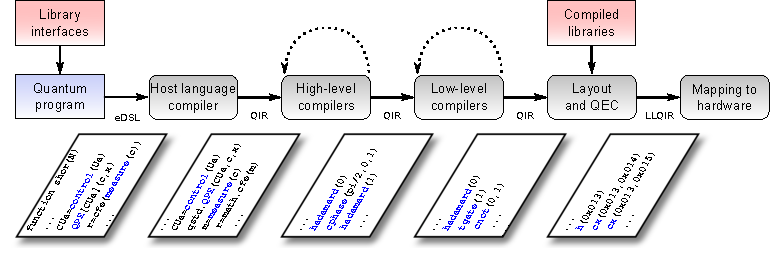
\includegraphics[width=\textwidth]{figures/coarse_toolchain}
\caption{The proposed toolchain for quantum programming: The quantum program is implemented in an embedded domain-specific language (eDSL) and then translated to hardware instructions using a series of compilers, which generate quantum intermediate representations (QIR) of the code. Pre-compiled libraries are linked against prior to creating the logical layout and applying error correction, since this will produce more efficient code. The resulting low-level quantum intermediate representation (LLQIR) is then mapped to hardware.}
\label{fig:toolchain}
\end{figure*}

The high-level quantum programming language may be one of several~\cite{gay2006quantum}:
some are based on C \cite{omer1998procedural} and others based on functional languages \cite{green13,wecker14}.
A compelling case can be made for an embedded domain-specific language such as Quipper \cite{green13} or LIQ$Ui\ket{} $\cite{wecker14} in order to leverage classical language and compilation features.
Both are functional languages, the former is embedded in Haskell and allows extensible data types and advanced programming constructs,
while the latter contains a domain-specific language embedded in F\#.
%In contrast to Quipper,  LIQ$Ui\ket{} $ also features simulators for noise and resource analysis, but neither allows for hardware backends.

The compilers of the stack will allow automatic translations to hardware instructions for specific backend quantum devices.  Auto-tuning of quantum libraries allows determination of the best representations for a given target backend and in turn can result in substantial cost savings in the final implmentation of the quantum algorithms on hardware.  Ultimately the software stack is designed to program and automate the control of a quantum computer, no matter the size of the algorithm or device.
A grand challenge for computer scientists and engineers will be to design the components of the quantum stack, such that the task of implementing a quantum algorithm and optimizing it becomes streamlined and efficient. The design will require leveraging the advances in the digital space, while also developing novel solutions for the quantum domain.

\section{Conclusion/Key directions}
\begin{enumerate}
\item    Establishing quantum supremacy on real hardware
\item     Software is in development
\item     Qubits are in development (see Rod's paper)
\item     Won't be bad for privacy, but will enhance it -- mention blind quantum computing here
\end{enumerate}



% needed in second column of first page if using \IEEEpubid
%\IEEEpubidadjcol


% An example of a floating figure using the graphicx package.
% Note that \label must occur AFTER (or within) \caption.
% For figures, \caption should occur after the \includegraphics.
% Note that IEEEtran v1.7 and later has special internal code that
% is designed to preserve the operation of \label within \caption
% even when the captionsoff option is in effect. However, because
% of issues like this, it may be the safest practice to put all your
% \label just after \caption rather than within \caption{}.
%
% Reminder: the "draftcls" or "draftclsnofoot", not "draft", class
% option should be used if it is desired that the figures are to be
% displayed while in draft mode.
%
%\begin{figure}[!t]
%\centering
%\includegraphics[width=2.5in]{myfigure}
% where an .eps filename suffix will be assumed under latex, 
% and a .pdf suffix will be assumed for pdflatex; or what has been declared
% via \DeclareGraphicsExtensions.
%\caption{Simulation Results.}
%\label{fig_sim}
%\end{figure}

% Note that IEEE typically puts floats only at the top, even when this
% results in a large percentage of a column being occupied by floats.


% An example of a double column floating figure using two subfigures.
% (The subfig.sty package must be loaded for this to work.)
% The subfigure \label commands are set within each subfloat command,
% and the \label for the overall figure must come after \caption.
% \hfil is used as a separator to get equal spacing.
% Watch out that the combined width of all the subfigures on a 
% line do not exceed the text width or a line break will occur.
%
%\begin{figure*}[!t]
%\centering
%\subfloat[Case I]{\includegraphics[width=2.5in]{box}%
%\label{fig_first_case}}
%\hfil
%\subfloat[Case II]{\includegraphics[width=2.5in]{box}%
%\label{fig_second_case}}
%\caption{Simulation results.}
%\label{fig_sim}
%\end{figure*}
%
% Note that often IEEE papers with subfigures do not employ subfigure
% captions (using the optional argument to \subfloat[]), but instead will
% reference/describe all of them (a), (b), etc., within the main caption.


% An example of a floating table. Note that, for IEEE style tables, the 
% \caption command should come BEFORE the table. Table text will default to
% \footnotesize as IEEE normally uses this smaller font for tables.
% The \label must come after \caption as always.
%
%\begin{table}[!t]
%% increase table row spacing, adjust to taste
%\renewcommand{\arraystretch}{1.3}
% if using array.sty, it might be a good idea to tweak the value of
% \extrarowheight as needed to properly center the text within the cells
%\caption{An Example of a Table}
%\label{table_example}
%\centering
%% Some packages, such as MDW tools, offer better commands for making tables
%% than the plain LaTeX2e tabular which is used here.
%\begin{tabular}{|c||c|}
%\hline
%One & Two\\
%\hline
%Three & Four\\
%\hline
%\end{tabular}
%\end{table}


% Note that IEEE does not put floats in the very first column - or typically
% anywhere on the first page for that matter. Also, in-text middle ("here")
% positioning is not used. Most IEEE journals use top floats exclusively.
% Note that, LaTeX2e, unlike IEEE journals, places footnotes above bottom
% floats. This can be corrected via the \fnbelowfloat command of the
% stfloats package.






% if have a single appendix:
%\appendix[Proof of the Zonklar Equations]
% or
%\appendix  % for no appendix heading
% do not use \section anymore after \appendix, only \section*
% is possibly needed

% use appendices with more than one appendix
% then use \section to start each appendix
% you must declare a \section before using any
% \subsection or using \label (\appendices by itself
% starts a section numbered zero.)
%


\appendices
\section{Suggested quantum applications/algorithms}

\begin{enumerate}
\item    Grover
\item     Linear systems
\item    Sampling
\item       Walks
\item       Etc.
\end{enumerate}

\section{Quantum architecture from a classical point of view}
\label{sec:box1}
\begin{enumerate}
\item      What do they take advantage of? (CALL OUT BOX)
\item  Parallelism - massive SIMD architecture
\item  Reversible
\item  Reduction (Prepare superposition, computer, reduce)
\item  There are only a limited number
\item  Give analogy to Map Reduce structure in SIMD setting
\end{enumerate}
% use section* for acknowledgement
\section*{Acknowledgment}


The authors would like to thank...


% Can use something like this to put references on a page
% by themselves when using endfloat and the captionsoff option.
\ifCLASSOPTIONcaptionsoff
  \newpage
\fi



% trigger a \newpage just before the given reference
% number - used to balance the columns on the last page
% adjust value as needed - may need to be readjusted if
% the document is modified later
%\IEEEtriggeratref{8}
% The "triggered" command can be changed if desired:
%\IEEEtriggercmd{\enlargethispage{-5in}}

% references section

% can use a bibliography generated by BibTeX as a .bbl file
% BibTeX documentation can be easily obtained at:
% http://www.ctan.org/tex-archive/biblio/bibtex/contrib/doc/
% The IEEEtran BibTeX style support page is at:
% http://www.michaelshell.org/tex/ieeetran/bibtex/
%\bibliographystyle{IEEEtran}
% argument is your BibTeX string definitions and bibliography database(s)
%\bibliography{IEEEabrv,../bib/paper}
%
% <OR> manually copy in the resultant .bbl file
% set second argument of \begin to the number of references
% (used to reserve space for the reference number labels box)
\bibliographystyle{IEEEtran}
\bibliography{references}
% biography section
% 
% If you have an EPS/PDF photo (graphicx package needed) extra braces are
% needed around the contents of the optional argument to biography to prevent
% the LaTeX parser from getting confused when it sees the complicated
% \includegraphics command within an optional argument. (You could create
% your own custom macro containing the \includegraphics command to make things
% simpler here.)
%\begin{IEEEbiography}[{\includegraphics[width=1in,height=1.25in,clip,keepaspectratio]{mshell}}]{Michael Shell}
% or if you just want to reserve a space for a photo:

%\begin{IEEEbiography}{Krysta Svore}
%Biography text here.
%\end{IEEEbiography}

% if you will not have a photo at all:
%\begin{IEEEbiography}{Matthias Troyer}
%Biography text here.
%\end{IEEEbiography}


% You can push biographies down or up by placing
% a \vfill before or after them. The appropriate
% use of \vfill depends on what kind of text is
% on the last page and whether or not the columns
% are being equalized.

%\vfill

% Can be used to pull up biographies so that the bottom of the last one
% is flush with the other column.
%\enlargethispage{-5in}



% that's all folks
\end{document}


